% !TEX root = $uni/master-thesis/thesis/main.tex
\documentclass[../discussion.tex]{subfiles}

\begin{document}
  \begin{figure}
    \begin{subfigure}{\textwidth}
      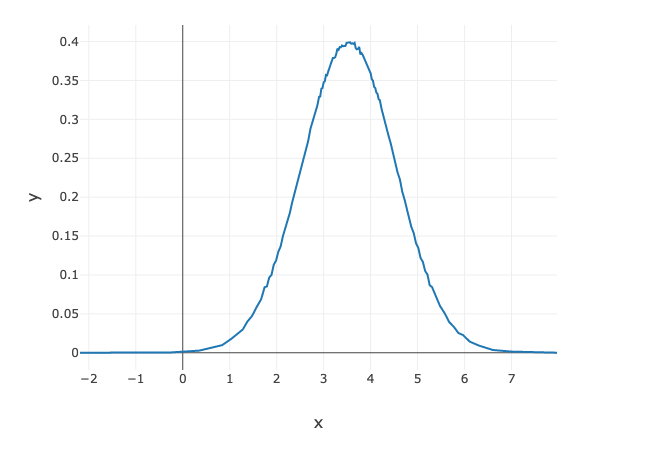
\includegraphics[width=0.9\linewidth]{graphics/2d-gauss-5root2mean-marg.png}
      \caption{2D, $\delta = \nicefrac{5}{\sqrt 2} \approx 3.5$}
    \end{subfigure}
    % \hspace*{\fill}
    \begin{subfigure}{\textwidth}
      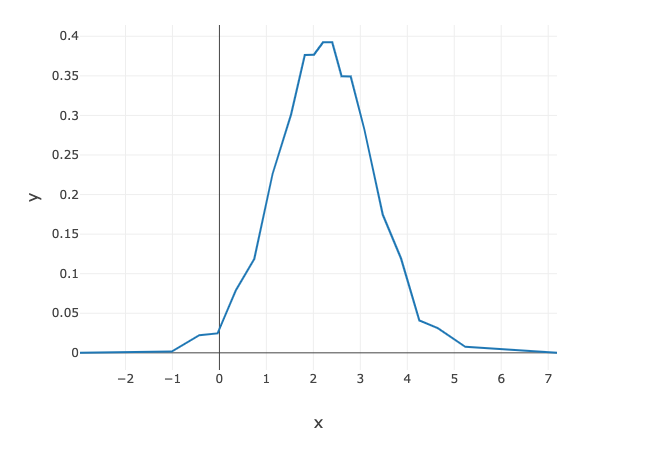
\includegraphics[width=0.9\linewidth]{graphics/5d-gauss-5root5mean-marg.png}
      \caption{5D, $\delta = \nicefrac{5}{\sqrt 5} \approx 2.2$}
    \end{subfigure}
    \caption{
      1D Marginalizations of histograms estimated from
      Multivariate Gaussian samples with mean $\delta \textbf{1}$ and
      identity covariance matrix.
      The marginalized histogram based on a bivariate Gaussian is much smoother,
      which is due to there being more leaves per dimension in that histogram before marginalization.
    } 
    \label{fig:marg-hists}
  \end{figure}
\end{document}